\documentclass[draftclsnofoot, onecolumn, 10pt, compsoc]{IEEEtran}

\usepackage[english]{babel}
\usepackage{amsmath}
\usepackage{graphicx}
\graphicspath{	{./}	}
\usepackage[top=0.75in, bottom=0.75in, left=0.75in, right=0.75in]{geometry}

\title{\textbf{I Heart Corvallis - Mobile Application\\Requirements Document}\\Capstone I\\Fall 2017}

\author{Omeed Habibelahian\\Bradley Imai\\Dylan Tomlinson}

\begin{document}
	\maketitle
	\begin{abstract}
		This document defines the perspective and scope of the I Heart Corvallis project. It defines key terms that will be used throughout the document, the final product's perspective and functions, the main user characteristics, and constraints that we will face throughout the project. It also defines the specific requirements necessary for completion of the project, such as the external interface requirements, functional requirements for each class of users, performance requirements, software system attributes, and our stretch goal for this project. It also includes a Gantt chart graphing the time frames for completing various aspects of the project.
	\end{abstract}
	\newpage

	\section{Introduction}
		\subsection{Purpose}
			This document will define the scope and requirements for completing the development of the I Heart Corvallis mobile application. It defines key terms central to the development of the application and its background, constraints and software complications that could influence completion of this project, and what key features will need to be implemented in the application before it can be considered completed. This document's intended audience is the Corvallis Community Relations office, who we are building this application for, and our instructors that will be grading and evaluating the project at the end of the year.

		\subsection{Scope}
			In this project, we will be producing the "I Heart Corvallis" mobile application. The app will showcase events happening around the Corvallis community, such as city council meetings, service and volunteer projects, and other community activities. It will also act as a passport for users to show that they have attended these activities. The app will give the user stamps upon completion or verification of attendance for each activity and will offer rewards to the user for accumulating enough stamps. On top of this, the application will showcase other resources available to community members. \\ \\
			The application will be available for Android devices and aims to inform members of the Corvallis community, both students and others, about various initiatives and resources around the community, as well as get community members more involved with community projects, events, and meetings by giving them an incentive to do so. \\ \\
			Another goal of the app is to help students be more aware of community events.  To accomplish this, the application will utilize the Google Maps API to show where events and various community resources can be found. The app will also include a separate page that will provide additional information about the city of Corvallis, such as links to website in the community and information about the Corvallis Community Relations (CCR) office and the initiative.

		\subsection{Definitions, Acronyms, and Abbreviations}
			\subsubsection{I Heart Corvallis} The application being developed in this project.
			\subsubsection{Corvallis Community Relations} A subset of the Office of Student Life. The Corvallis Community Relations office is the leader of the I Heart Corvallis initiative and the client for this project.
			\subsubsection{Stamp} In-app verification that the user has attended a particular community activity. Some activities will be worth more stamps than others.
			\subsubsection{IDE} Integrated Development Environment; a software application that provides comprehensive facilities for software development. An IDE typically consists of a source code editor, build automation tools, and a debugger.
			\subsubsection{Xcode} The official IDE for software development on Apple's mobile and desktop operating systems.
			\subsubsection{Android Studio} The official IDE for software development on Google's Android operating system, built on JetBrains's IntelliJ IDEA software and designed specifically for Android development.
			\subsubsection{Database} A structured set of data held in a computer, especially one that is accessible in various ways.
			\subsubsection{Node.js} A runtime environment used for executing server-side JavaScript code.
			\subsubsection{Meteor} A web framework written in Node.js that allows for the production of cross-platform code between Android, iOS, and webpages.
			\subsubsection{MongoDB} A document-oriented database program.

		\subsection{Overview}
			The client of this application is the Corvallis Community Relations office. They have asked us to create a mobile application to aid them to list the various community events, projects, and meetings being put on by different organizations, authenticates the user, successfully tracks the events they engage in, and provides rewards for completing enough community activities. The I Heart Corvallis mobile application will be dedicated to OSU students and community members.

	\section{Overall Description}
		\subsection{Product Perspective}
			This product will be visually similar to that of other Oregon State University mobile applications and desktop pages, but functionally it is completely independent of any other systems. The Corvallis Community Relations office wants to use the I Heart Corvallis application in conjunction with their OSU Corvallis Community Relations website, but the two will not be directly reliant on each other.

		\subsection{Product Functions}
			When the user first opens the application, it will show the login page. This page asks if the user is an OSU student or a permanent resident. Students will be redirected to the ONID login screen for authentication, while permanent residents will be asked to log in with their username and password. They will be given the option to create a username and password if they have not previously done so. \\ \\
			If the user is logging in for the first time, the app will display a short survey with a few questions for users to answer before their home page loads. Once the user has logged in, the app will display the home page, which provides quick links to the user's passport, the list of upcoming events, the stamp leaderboard, prize page, community resources page, and a page about the creators of the application and information about the I Heart Corvallis initiative. \\ \\
			Both the event list page and the passport page list community events in chronological order. Non-timed, location-based events will be listed first, followed by the events with a specific date and time being listed afterwards. Each event's information box will show the event title, location, and the date and time if applicable. The event list page will also show the number of stamps that each event is worth, whereas the passport page will show an indicator of whether they attended that event or activity, and how many stamps they received for doing so. \\ \\
			The user can press on an event to pull up the detailed information page for that event, which will include a picture for the event, as well as the event title, location, date and time if applicable, description, and any relevant links provided by the event host. The passport page will also provide a button that indicates the user's current level, which will be determined by the number of stamps they have accumulated. There will be bronze, silver, and gold levels, each of which will correspond to different prizes. When the user presses the button, they will be taken to a page that lists the available prizes, separated by level. This prize page will also be accessible from the home page. \\ \\
			The community resources page will show other resources available to community members, as well as a link to the Corvallis Living Guide website. This page will also include a Google Map that will display various community establishments such as entertainment locations, grocery stores, restaurants, shopping locations, and city offices. The "about" page will provide a short description of the app and its purpose, as well as information about the Corvallis Community Relations office. \\ \\
			The Corvallis Community Relations office will also have access to a back-end page that they will use to add, edit, and remove events, as all events will have to be approved by the office before being added to the application's event list, and the office will have the sole authority to post, edit, and remove these events. They will also be able to edit survey questions and other pages throughout the app, as well as add or remove stamps for users. They will be access this page through a special administrative login. \\ \\

		\subsection{User Characteristics}
			The intended users of the I Heart Corvallis app are OSU students and permanent residents of Corvallis. The app does not require any special technical or educational expertise, as it will be designed for anyone to be able to navigate without needing to learn any new technical skills. As long as the user knows how to use a mobile application, the app will be designed to be simple enough for even non-tech savvy users to navigate.

		\subsection{Constraints}
			There are a couple of constraints that can potentially limit our options as far as project completion is concerned. The Corvallis Community Relations office wants the application to be developed for both Android and iOS, but Android and iOS apps are usually coded in different languages and tested in different IDEs. Therefore, efficiently coding for Android and iOS simultaneously in a cross-platform fashion will be a challenge. Because of this, our primary focus will be on completing the Android version of the app, and if time allows after completing the Android version, we will build the iOS version. \\ \\
			Another constraint is the availability of testing environments across multiple desktop platforms. While Android Studio is available for both Mac and Windows, Xcode is a Mac-exclusive IDE, and not everyone on the development team has a Mac computer. Therefore, we will have to find the best way for all three of us to build the iOS version of the application.

		\subsection{Assumptions and Dependencies}
			The main factor that will influence the requirements for this project is whether or not we can successfully build the application in a cross-platform fashion. The Corvallis Community Relations office has mentioned Meteor, or MeteorJS, as an option for cross-platform implementation of the app. Meteor would allow us to build the application using JavaScript and would allow for synchronous cross-platform implementation across both Android and iOS without the use of either Android Studio or Xcode. However, Meteor uses MongoDB as its database, which we have historically found to be more difficult than other databases such as SQL. Meteor is also a platform that none of us on the development team have prior experience with, whereas we do have experience with IDEs like Android Studio.

	\section{Specific Requirements}
		\subsection{External Interface Requirements}
			\subsubsection{User Interfaces}
				When the application is opened for the first time, it will display a log-in screen. There will be two log-in systems implemented into the app, as the login for students will be separate than for permanent residents. \\ \\
				The app will display the home page whenever the user reopens the app. This page will display quick links to other pages, such as the user's passport, stamp leaderboard, prizes available, and a page about the creators of the application and the I Heart Corvallis initiative. \\ \\
				The passport system will allow the user to accumulate points, or "stamps," after completing or attending various community activities and events, and the user will be able to win prizes for accumulating enough stamps. \\ \\
				The application will also be connected to two databases, one for events and one for user account information. The event database information will hold all of the information for each event being advertised by the app. The user account database will hold the user's login credentials, which will be kept secret to minimize the risk of the wrong user getting access to someone's account, as well as their passport information. \\ \\
				The application will provide a map that displays the locations of important and notable community resources, events, and activities, as well as sources of entertainment, restaurants, shopping centers, and city offices. We will utilize the Google Maps API to implement this map into the application. The locations of the events advertised in the app will be shown on the map as well, and the user will be able to click on a pin on the map for more information about the event, activity, or establishment that pin represents.

			\subsubsection{Hardware Interfaces}
				The only hardware restriction on the application is that it will initially be exclusively available on the Google Play Store for Android devices. Our stretch goal is to build an iOS version of the application and publish it to the App Store as well. Other than this, the application itself doesn't have any designated hardware interfaces.

			\subsubsection{Software Interfaces}
				The application will use the user's smartphone's GPS to track their current location to check if they are at the location of a community event or activity. It will also require an internet connection to retrieve event information from the event database and retrieve the user's information from the account database.

			\subsubsection{Communications Interfaces}
				Communication between different sections of the app is vital for the app's success, so links and buttons will have to take the user to the correct page. Links will redirect to the smartphone's Internet browser, pressing on an event box will bring up more information about that event, and quick links will redirect to their respective full pages. The underlying operating system will also be vital to successful communication between sections of the app.

		\subsection{Functional Requirements}
			\subsubsection{Student and Permanent Resident Users}
				Student users and permanent resident users shall be able to:
				\begin{itemize}
					\item View the list of events happening around Corvallis (both general information and detailed descriptions)
					\item View their passports
					\item Check in using their current location and enter a code to receive a stamp for time-based events
					\item Check in using their current location to receive a stamp for location-based events
					\item View a map of community establishments
					\item (Permanent residents) create an account with a username and password and log in
					\item (Students) Log in using their ONID account (no need to create an account; ONID is the account)
					\item View available prizes
					\item See and answer survey questions upon their first login (student survey will be different than the resident survey)
					\item View a leaderboard of who has accumulated the most stamps
					\item View an informative page about the I Heart Corvallis initiative, the creators of the app
					\item View a page informing the user about various resources available in the community
				\end{itemize}
			\subsubsection{Administrative Users}
				Administrative users shall be able to:
				\begin{itemize}
					\item Add, edit, and remove events
					\item Edit survey questions
					\item Edit the community resources page
					\item Edit the "about us" page
					\item Log in to edit content via their own special administrative login page
					\item Add and remove stamps for users
				\end{itemize}

		\subsection{Performance Requirements}
			The application will support up to 20 simultaneous users. The user will not have to input very much information, as the app will generally show them upcoming community events and activities, how much of their passport they have completed, what prizes they can win and how they can redeem it, and various community resources available to them.

		\subsection{Software System Attributes}
			\subsubsection{Reliability}
				The application will have a user interface that 8 out of 10 users will be able to navigate without difficulty. The application will also function without crashing 95\% of the time.

			\subsubsection{Availability}
				The application will initially be available for Android, and if we can meet our stretch goal, it will be available for iOS upon launch as well. The application will require an Internet connection to function properly. If the Internet connection is lost or the app crashes, the app will recover any account and event information that had already been successfully stored in the database.

			\subsubsection{Security}
				For OSU students, the authentication system will be the same as for other services that require an ONID login for authentication. The student will have to log in with their ONID username and password to be able to access the app. To protect student accounts, we will not store their ONID password in the account database, as the ONID interface itself authenticates the user. We will only store their ONID username. For permanent residents, we will encrypt their password to prevent potential hackers from obtaining users' passwords, and the encrypted password will be stored in the database.

			\subsubsection{Maintainability}
				We will create separate functional and formatting code files for each page in the app. This way, the app will be modularized in such a way that editing the makeup of one page will not affect the behavior of the other pages of the app. This will result in many code files being created but it will allow us to edit one page independent of the other pages.

			\subsubsection{Portability}
				Since the primary programming languages for Android are different than for iOS, a majority of our components and code will be host-dependent. About 85\% of the application's components will include host-dependent code, and about 80\% of the total code for this project will be host-dependent. This is due to the fact that Android apps are generally coded in Java and XML, while iOS apps are generally coded in Objective-C and Swift. For the databases, we will code in SQL and PHP, both of which are portable programming languages.

		\subsection{Stretch Goals}
			Our main stretch goal is to build and publish an iOS version of the application, complete with all of the features available on the Android version of the application.

		\subsection{Timeline}
			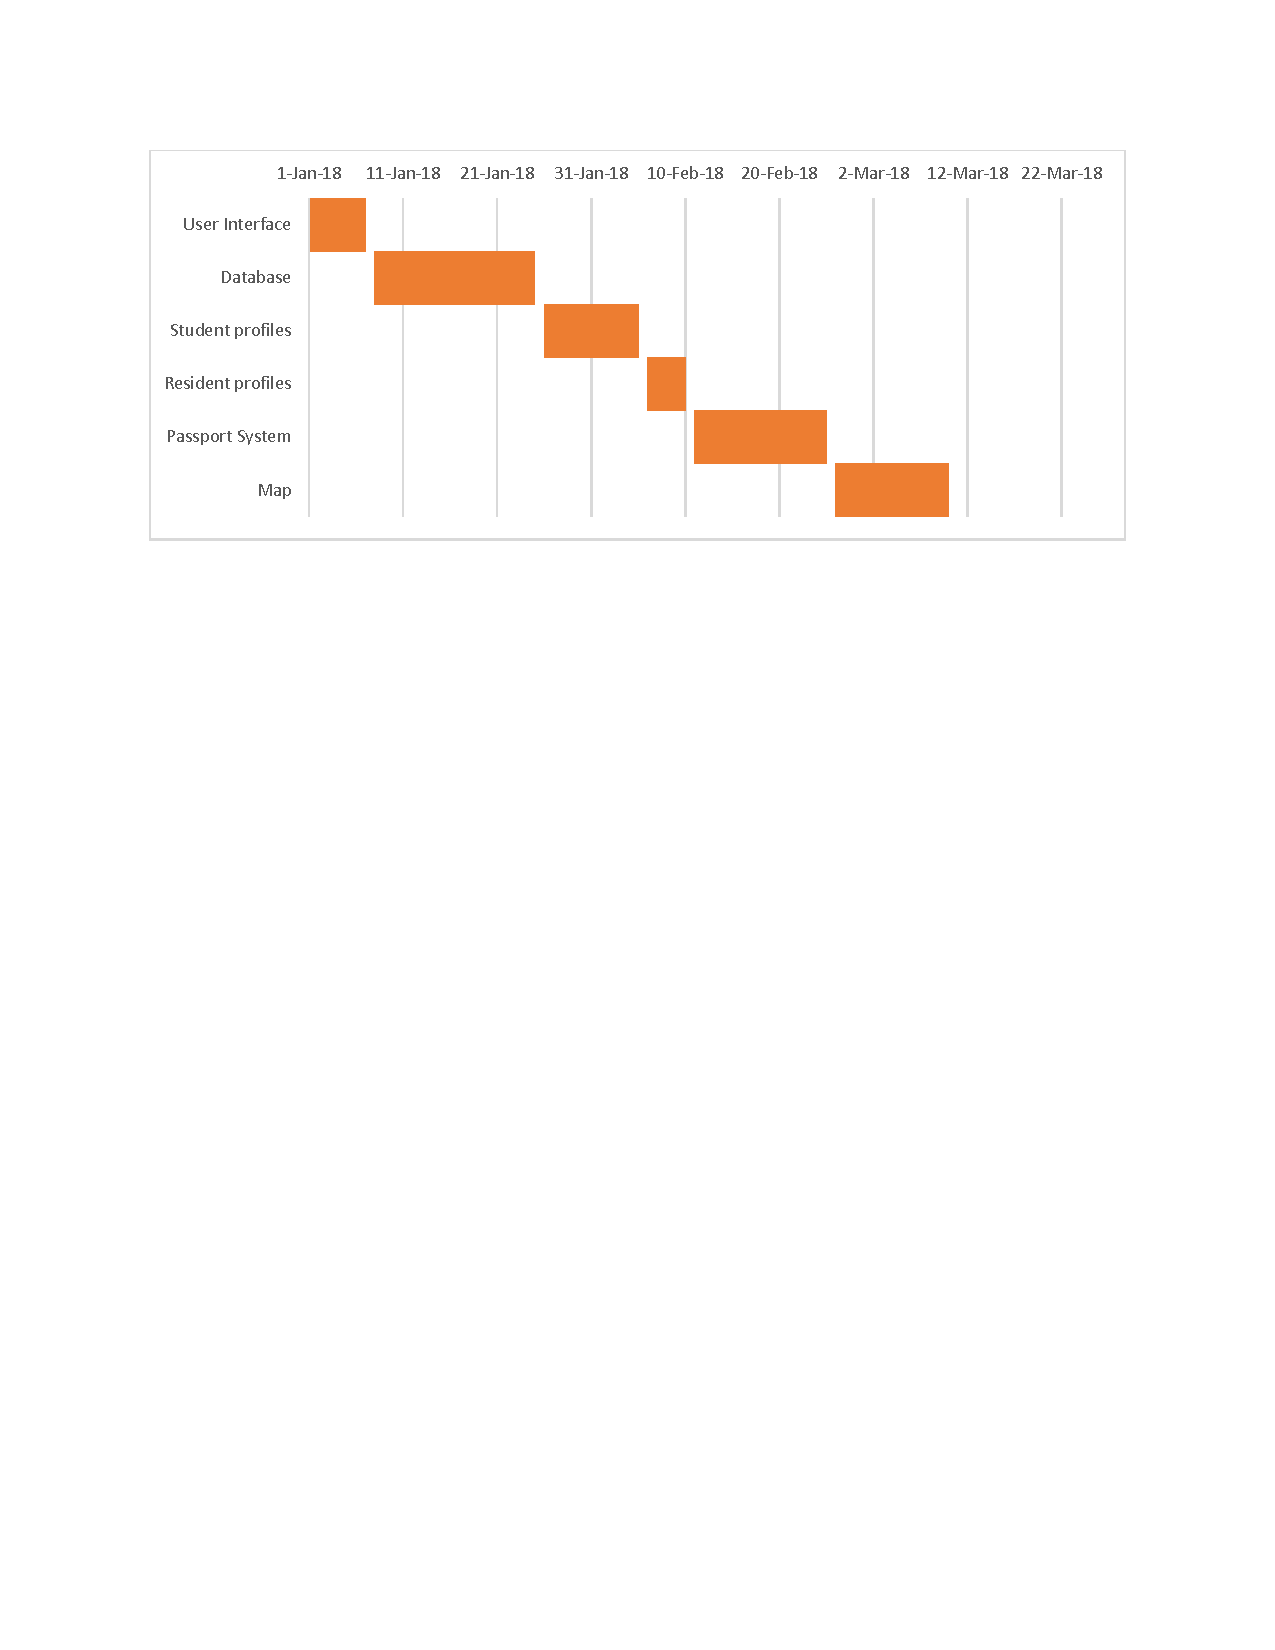
\includegraphics[width=\textwidth]{GanttChart.pdf}

\end{document}
